%
\section{Literature Survey}\label{sec:literature survey}
%
This is the last chapter of this thesis \cite{tur38}.
%
\subsection{Evolution of Vulnerability Analysis}
Vulnerability analysis is an important operation to perform in all domains which also includes the software product. One single vulnerability can cause a catastrophe in an active system and which can be an open gateway to the attackers to exploit the system. A good vulnerability assessment should define, identify and categorize the issues in the component. 
Neumann and Parker say that the new vulnerabilities of IT systems are evolved from the attacks that happened in the past by using long-known techniques[21]. Therefore building a strong and secure application is merely an impossible task or will be more expensive. Earlier the vulnerability assessment happens manually  in all organizations where this is a huge and overwhelming work for the IT security teams. 
\paragraph{}
All the newly identified vulnerabilities should be stored in excel or a CSV file for later use. When compared to the no. of vulnerabilities today, the 90’s and late 2000 had very less number of vulnerabilities. The early vulnerability scanning software just gives a simple report of found vulnerabilities in the system and later this report has to be given to the IT security team to analyse the possible threats of the vulnerability. Then the report is sent to higher authority for a review and approval. This is such a manual process which has been used earlier to detect vulnerabilities in an active system[22]. Manual scanning and repair strategies would soon become impractical as the number of vulnerabilities grew in following years and the necessity of vulnerability management became more apparent to companies. Now the future of vulnerability analysis is focussing on fully automated assessment.
\subsubsection{Benefits}
Lutz Lowis describes that attackers may usually repeat their exploits by reusing a susceptible service[20]. Despite many old and new threats there are few advantages to performing vulnerability analysis operations. Here are some advantages that can be achieved through a vulnerability assessment[20][22][23]:
\begin{description}
	\item [$\bullet$]A vulnerability analysis can identify all the possible vulnerabilities in the system where this can be identified by both organization and the attacker(hacker) if they use the same software for scanning. The organization has a higher advantage by fixing this issue before the attackers initiate. 
	
	\item [$\bullet$]If the IT security person conducts a regular scanning of the system, the scanning can give the level of risk available in the system. So this helps to figure out the health of the overall system.
	
	\item [$\bullet$]Vulnerability assessment will save money and time because if an organization or individual fails to complete the vulnerability analysis procedure, there is a greater possibility that an attacker will be able to exploit the system, resulting in the system having to be rebuilt.
	
	\item [$\bullet$]The previous evaluation reports will be useful in improving the present system in the future.
\end{description}
\subsubsection{Vulnerability Attacks}
A vulnerability is an attribute of a software component that has a potential of exploiting or damaging an active system. Most of the vulnerabilities have a high tendency of causing damage to security policy by internal or external persons(hacker or insider). There is a past event which happened in 2017 where a big data breach occurred in Equifax. This data breach caused more than 100 million user data to be leaked[4]. In this vast area of IT there are still new and unknown vulnerabilities emerging everyday.
\paragraph{}
Ryohei Koizumi and Ryoichi Sasaki have found that whenever a vulnerability assessment operation takes place the IT security team should always use the latest scanning tool because sometimes the old softwares is effective against some small virus threat but it does not exploit the vulnerability[24]. There are some vulnerability attacks which have to be focused more because these type attacks are listed as high in risk level. Here are some major attack types that are focused by few researchers[25]:
\begin{description}
	\item [$\bullet$ Configuration-based:] This type of vulnerability occurs when there is a misconfiguration in the system or running any unwanted services in the background. The configuration-based vulnerability has a major weak point where the hackers can easily get into the organization network and try to find the active system by any form of misconfiguration. This type of vulnerability is based on weak management protocols, weak permissions and weak encryption.
	
	\item [$\bullet$ Security patches:] A security patch is an important update for all active systems because a role of a security patches is to fix or remove the flaw or issue which is found from the vulnerability report. The software patches play a vital role in rectifying and fixing the components for both commercial software and open-source software components. Generally the security patches will be released every month for example Microsoft sends security patches to its windows operating system every month. A system which fails to update their security patches will lead to major security breaches. As everyone knows, the best example of security patches failures is ransomware which is called wannacry[26].
	
	\item [$\bullet$ Zero-Day Vulnerability:] This is the most difficult vulnerability to rectify and fix the issue, this is because the vulnerability is new and unknown to the organization. The attackers will take advantage of this loophole and will cause a major security risk. The term “Zero-day” is used because the vendor was unaware of the threat which affected the software and the vendors had “0” days worked on the security patch or fixing the vulnerability.
	
	\item [$\bullet$ Faulty Open-Source Package:] This the vulnerability where hackers were using it for several years. Generally the hackers used to inject a credential sniffer inside a very useful common library or package. This kind of attack happens when the vendor doesn’t update the open-source packages regularly. This threat will stay in the package for several days or until it is found by the vendor.
\end{description}

\subsubsection{Types of Vulnerability Analysis}
The vulnerability analysis is also called vulnerability assessment where the main intended purpose of this is to keep the organization safe from the digital threats. This is a methodology which is used to find the IT application and the infrastructure. It also involves intense scanning by the security expert or team of the organization. There are few types of vulnerability analysis which are used exclusively for some part of IT:

{\bf Network-based Analysis:} A network-based analysis is a mechanism to identify the network defects and issues in the network. They mostly scan and analyze the network endpoint and device network for security issues. The failure of vulnerability analysis will give an opportunity to the hackers to take advantage of the network issue. The organization will invest more time to improve their existing framework which is used for network vulnerability analyses. In 2008 Hai L Vu etl, developed a vulnerability analysis framework for scanning network vulnerabilities and along with that they have also proposed a scalable algorithm. Both framework and algorithm are used to evaluate the network vulnerabilities without generating a full-scale graph[27]. This figure gives the results of each network component used in the network by using the framework. The results come with a brief description about the effects of the listed vulnerability. These information about the vulnerabilities have been taken with the help of vulnerability databases[27].

\begin{figure}[h!]
	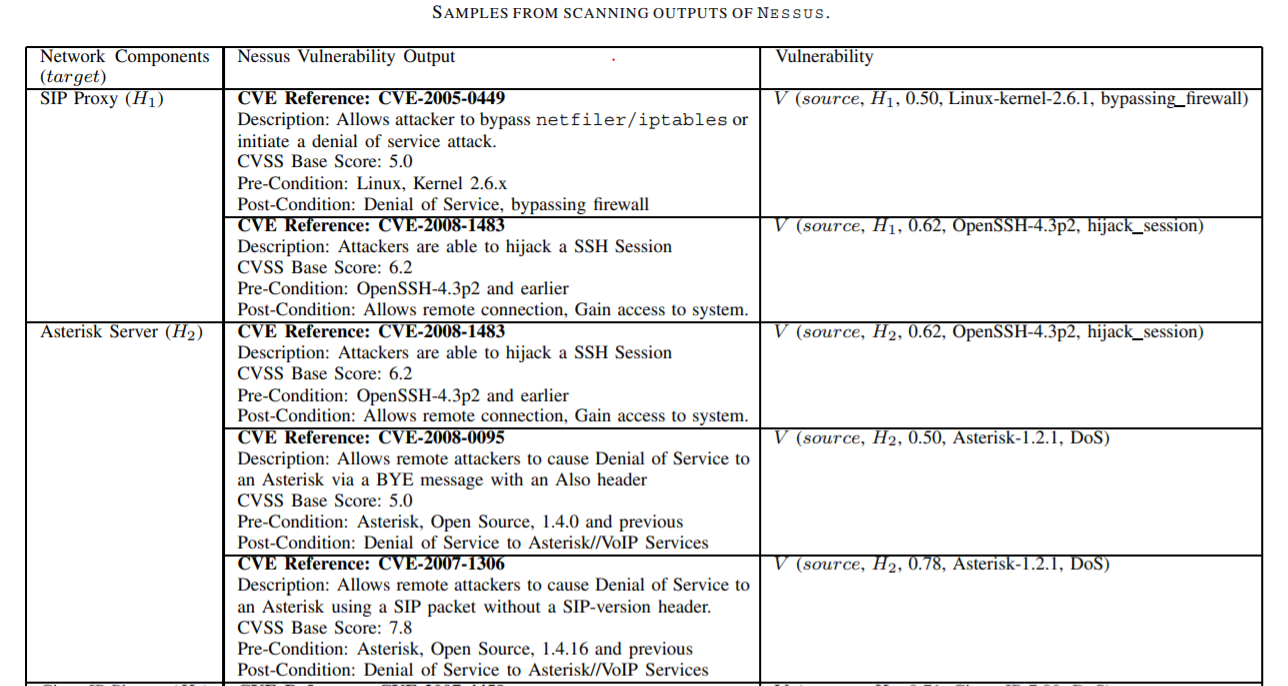
\includegraphics[width=15cm]{includes/networkanalysis.png}
	\centering
	\caption{Sample results of the network vulnerability analysis framework[27]}
	\label{fig:networkanalysis}
\end{figure}

{\bf Host-based Analysis:} Sometimes a vulnerability can be found in the vendor's resources and with this vulnerability there are high chances where even an insider can be an attacker for the system. The attackers mostly cause damage by making an improper configuration setting in the host.This vulnerability assessment takes place in servers, workstations or other network hosts. The host-based analysis will give a detailed insight of configuration settings in the network, patches and update history. The insight which is gathered from the analysis will also give us the potential damage caused by the attackers or intruders. Anil Sharma et. al. created a software tool “Ferret” by using perl language that simply identifies the vulnerabilities present in the host[28]. This software tool helps the system administrator to identify the vulnerabilities and take action based on the threat. The host vulnerability is checked by using a different plug-in module and the end output will also mention which plug-in module is used for the assessment.

{\bf Database Analysis:} Misconfigurations occur often in databases and Big Data systems. Database vulnerability analysis is mainly used for identifying the available risk in the databases. The most common risks are missing patches, weak passwords and default vendor accounts[29]. Sartaj Singh described the importance of inherent dangers of the database like how data theft is happening in the internet era and he also mentioned that the existing encryption methods are not fool proof for the high end professionals[31]. A vulnerability attack can exploit file permission, database configuration files and also have potential to steal sensitive information like credit card details, personal details, etc. There is still research going to secure the database more effectively and efficiently. In 2008 Ghassan Jabbour and Daniel A. Menasce presented a framework that provides a self protection to the database from unauthorized or intensional security parameter changes and also they proposed that this framework can be implemented in an Oracle 10g Release 2 database[32].

{\bf Application Analysis:} Vulnerabilities are frequently identified in third-party apps that are built and managed. The vulnerability assessment is important to an organization’s security team because they have to identify the vulnerability in the application before it exploits the system. This process is used to identify vulnerabilities which are misconfiguration in applications, outdated software packages and weak authentication. Sultan S. Alqahtani[33] has researched a modeling approach that improves traceability and trust in software products by linking the security knowledge with the software artifacts. He also introduced a scanner called  Semantic Global Problem Scanner(SE-GPS) which is created by integrating the modeling approach and with the modeling approach the tool can now link the NVD[13] security database to the maven build repository. 
\paragraph{}
The application vulnerability analysis is an important security process to be considered by the organization. The process's main goal is to identify the vulnerability and report it to the security authority to mitigate it before the vulnerability exploits the system. Most application vulnerability analysis tools use the proper guidelines to make a good scanning tool. Here is the main guideline that a good vulnerability scanner tool should use[34]:
\begin{description}
	\item [$\bullet$ Setup:] The setup should begin with a proper documentation about the application, with perfect security permissions and configuration tools.
	
	\item [$\bullet$ Test Execution:] Run the scanner tool which can be an existing tool or a self created one. The scanner should identify all the software packages and its dependencies used inside the software product.
	
	\item [$\bullet$ Vulnerability Analysis:] Once the execution is finished, the extracted software packages and its dependencies should be analysed by using any existing vulnerability databases like NVD, ISS(Internet Security Systems) , etc. each software package is searched in the database by using its name and version.
	
	\item [$\bullet$ Reporting \& Remediation:] After the previous process, the analysis will give a proper report of each software package. The report includes the risk level of each package which is categorized as LOW , MEDIUM and  HIGH. Sometimes the report will also provide a brief description of the threat. The remediation action is taken by the security department of the organization. Mostly the remediation will have two possibilities which is to change the version of the package or to find an alternate software package.
\end{description}
\subsubsection{Vulnerability Databases}
A vulnerability database is a collection of information about all known defects of a software application. This database is aimed to maintain all the information like name, version, threat description, level of risk and history of the components. New vulnerability information is generated every day to be fed into the database so that it can be a known vulnerability for the future users. Each information is reviewed properly by the respective vulnerability database before being generated into the database[35]. The vulnerability information can be given by the software owner, security researcher and public users of a software. Most of the databases use \acs{CVE}’s information to be integrated with the vulnerability database[14]. The Common VUlnerabilities and Exposures(\acs{CVE}) is a program which is owned by the MITRE’s corporation. The \acs{CVE} is built for one main purpose which is to identify, describe and catalog the cybersecurity vulnerabilities.
\paragraph{}
There are a lot of public and private vulnerability databases which are maintained by both government and private organizations. Each database is selected based on the user's preference of choice where some like to go with public or proprietary databases. In most cases the user’s always prefer to use the public database due two main reasons, it is maintained by the government and its open-source. Here is a list of major vulnerability databases[20]:

{\bf NVD:} Among all the databases National Vulnerability Database is the most commonly used database by the users. The NVD was first found in 2005 by the US National Institute of Standards and Technology(NIST)[13]. Most of the known vulnerabilities for both commercial and open-source are fed into the NVD databases and that is why NVD is one of the largest and most efficient vulnerability databases. NVD is a completely open-source project so that anybody can use it without any restrictions. The NVD integrates CVE’s information for every component present inside the database[14]. The CVE is mapped in the database by using the CVE id so that the user can easily retrieve the information from the CVE dictionary if needed. All the data stored in the database have a unique id for each vulnerability, date of history and short vulnerability description. The NVD also integrates CVSS(Common Vulnerability Scoring System) information to each vulnerability.
\paragraph{}
The fig 1.3 will give a clear idea about how components can be searched in the NVD database. The result list will be provided based on the keyword entered in the search bar along with information like CVE id, short summary of the vulnerability and CVSS score.
\newpage
\begin{figure}[h!]
	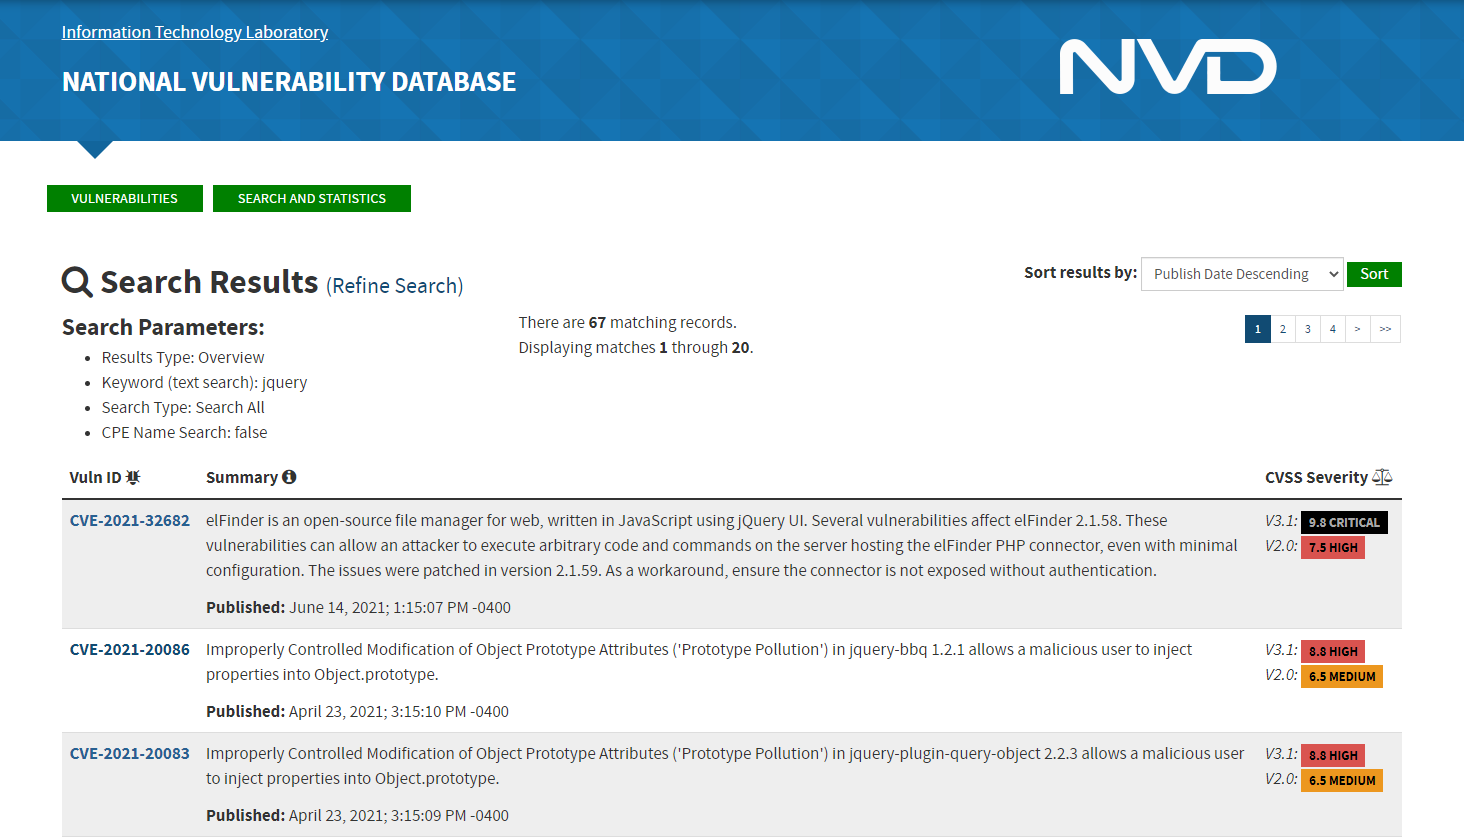
\includegraphics[width=15cm]{includes/nvd.png}
	\centering
	\caption{NVD result for “jquery” component.}
	\label{fig:nvd}
\end{figure}

{\bf SecurityFocus:} The SecurityFocus is a traditional news portal where the community discusses the new security issues of the vulnerabilities. The Bugtraq is the most common product of the securityfocus. The Bugtraq tool is exclusively used to list all topics about the security issues, like new vulnerabilities, exploitation methods and security related announcements by the vendor. Bug traq was created in 1993 by Scott Chasin. On Tuesday, May 14th, 1996, Aleph One gained control of BugTraq. BugTraq has evolved into a well-respected security mailing list with over 27,000 subscribers over the years[36].
\paragraph{}
Ashish Arora et al[37] made an empirical analysis on Vendor’s patching behaviour by evaluating the gap between the date of vulnerability disclosed and date of security patch rollout. They have discovered that a vendor takes an average of 29 days to fix the issue from the date of vulnerability is disclosed. To achieve this, the authors have compiled data from Securityfocus and CERT/CC. The author also confirmed that the vendors take more time to fix the vulnerabilities which they get from CERT/CC. This means the authors say that the vendor responds more faster to SecurityFocus vulnerabilities than the CERT/CC. The results of SecurityFocus will give information like Bugtraq ID, its class of error, publish date and its CVE ID. It also uses CVE information to list all vulnerabilities and give a discussion forum to report any further errors after the security patches. Figure 1.4 is an example of the vulnerability publication of SecurityFocus.
\newpage
\begin{figure}[h!]
	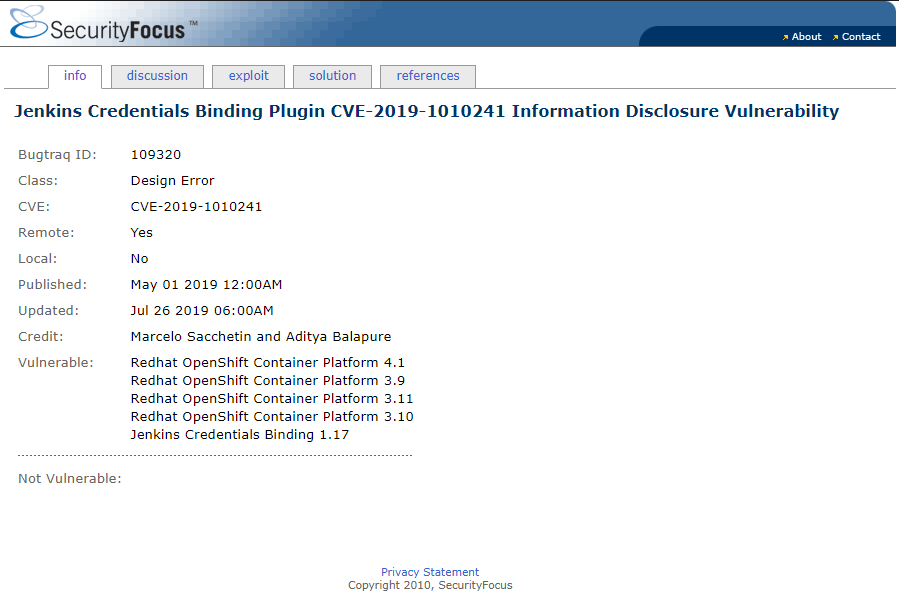
\includegraphics[width=15cm]{includes/securityFocus.png}
	\centering
	\caption{Example of vulnerability publication by SecurityFocus[38].}
	\label{fig:securityFocus}
\end{figure}

{\bf IBM X-Force:} The IBM X-Force is an elite team of security experts that contains the world's most talented hackers and incident responders. They are dedicated to resolving some of the toughest cybersecurity challenges in the world. The IBM X-Force is led by former FBI Cybercrimes Division Assistant Director Chris Soghoian, who brings over 20 year experience to this role. Unlike NVD, the X-force is a proprietary software whereas NV is completely open-source. Despite being a proprietary software, the X-force gets its vulnerabilities information from the CVE dictionary. Apart from this, X-force is also providing API services for this software. X-force requires an IBM id to get full access, which will be a paid service later. X-force also uses CVSS scoring system to give a clear risk level of the vulnerability. Though it is a proprietary database not many researchers will use this database for research purposes. Figure 1.5 is an example of vulnerability publication by IBM X-Force[39].
\newpage
\begin{figure}[h!]
	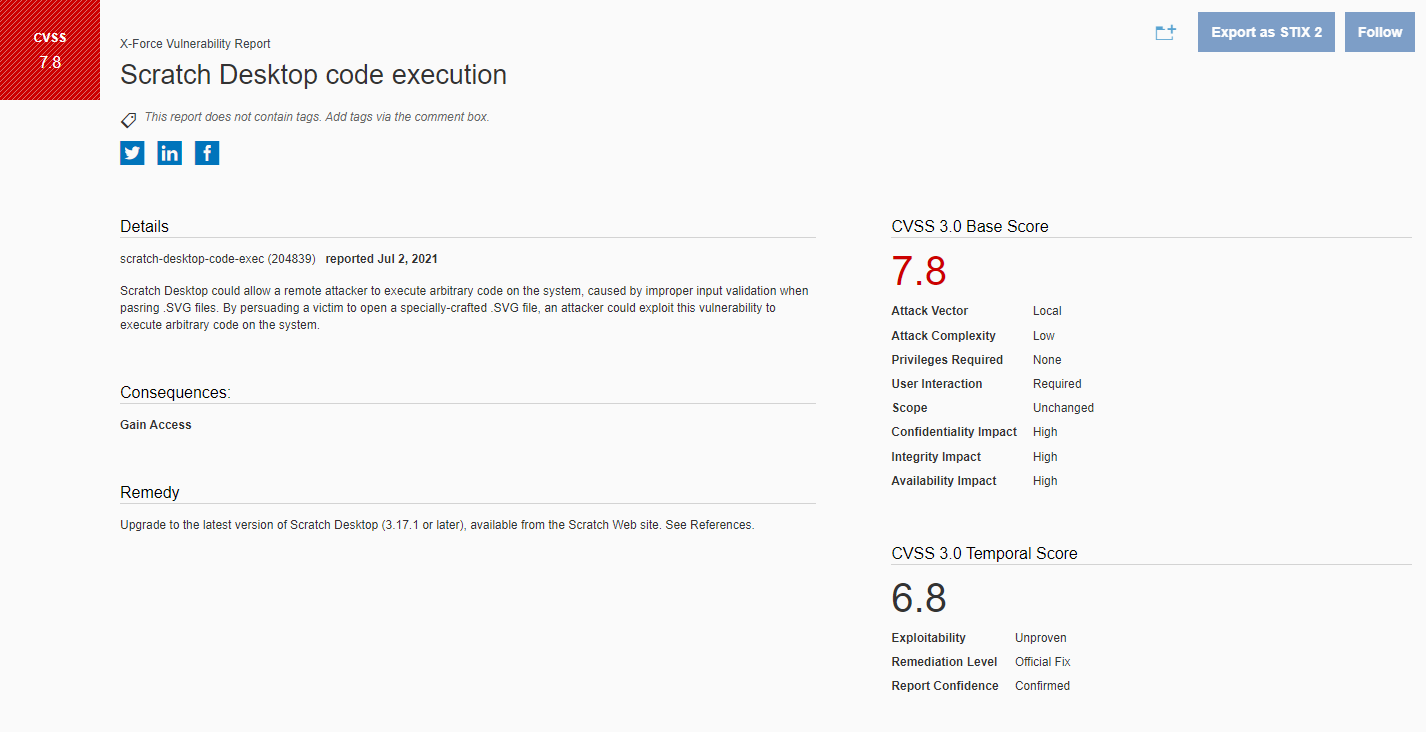
\includegraphics[width=15cm]{includes/ibm.png}
	\centering
	\caption{Example of vulnerability publication by IBM X-Force[39].}
	\label{fig:ibm}
\end{figure}

{\bf CERT/CC:} The CERT/CC stands for Computer Emergency Response Team Coordination Center[40]. CERT is also one of the databases which provides information about ongoing vulnerabilities and it also tries to resolve incidents like data breach and denial-of-service-attacks. CERT/CC was founded in 1988 by Carnegie Mellon University in Pittsburgh, Pennsylvania and supported by the Defense Advanced Research Projects Agency, which was part of the U.S. Department of Defense[41]. The main characteristic of CERT/CC is to resolve the security incident and try to regain control and minimize the damage. Later on they will assist to report the incident response to prevent the issue from happening again. Figure 1.6 is an example of vulnerability publication by CERT/CC.
\newpage
\begin{figure}[h!]
	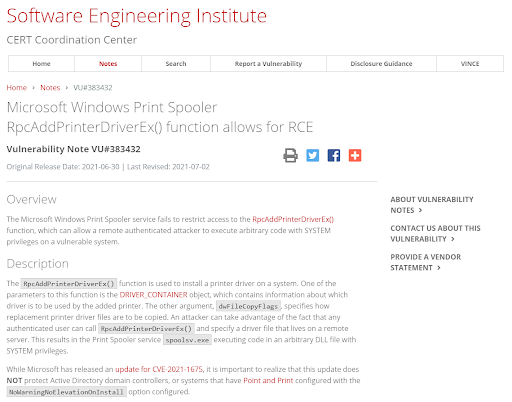
\includegraphics[width=15cm]{includes/cert-cc.png}
	\centering
	\caption{Example of vulnerability publication by CERT/CC[41].}
	\label{fig:cert}
\end{figure}

In general, the main goal of the incident response team is to protect the organization from any sort of vulnerability which can be software, network or cybersecurity related issues. The CERT/CC follows a universal incident response model which is “protect, detect and respond” [42].
\begin{description}
	\item [$\bullet$ Protect:] The first step of this model is to protect the organization by taking some security measures before the incident happens.This model focuses on more protecting than reacting to it for example, creating an incident response plan, providing security awareness, performing risk analysis, etc.
	
	\item [$\bullet$ Detect:] This is a process which happens before responding to the vulnerabilities. A proper response can be given to solve the vulnerability if the detection of the vulnerability is proper. Sometimes the duration of detection might take a month, week or a day and it completely depends on the security incidents. Before performing a detection strategy the responsible person should be able to provide solutions for example, applications which run often, how normal network traffic looks, what the network protocol should be avoided, etc. The common technique of detection is routers, firewalls, network monitors, etc.
	
	\item [$\bullet$ Respond:] Once the security incident is detected then the final step will be providing the perfect solution to it. Generally providing a response to the security incident has a few steps. The first step will be getting the information about the security incident from the vendor or business partner. The next step is the team will analyse the information to find quick and effective solutions to it. Once the solution is found, the team will create an immediate strategy to stop the issue before it causes more damage. The last step will be responding to the incident and will be published to others so that the affected users can regain control.
\end{description}

\subsection{Data Scraping}
Data scraping is an automation process which is used to extract data from files, websites, databases or any application. With the help of data scraping a user can get a huge amount of relevant data such as product reviews, business contact information, social media post or specific content from a file. The above mentioned content can be extracted by using existing data scraping tools or can build a custom program with the help of programming language support. Sometimes data scraping is also called web scraping just because it is widely used in the web domain. After the birth of the world wide web in 1989 the businesses started showing interest in creating websites to show their business related information such as product details, upcoming events and contact forms. From then the evolution of data scraping has been tremendous whereas now the data scraping techniques are used in cloud-based applications. Ram Sharan Chaulagain et al proposed a cloud-based web scraper architecture that can handle storage and computing resources with elasticity by using Amazon web service[43]. This architecture was proposed by concerning the previous drawbacks of scraping large amounts of data such as reliability of data scraping, storage issue of large datas and intensive computation. So therefore this clearly explains that large amounts of data cannot be extracted by using the traditional data scraping methods.

\subsubsection{Types of Data Scraping}
Generally data scraping techniques are used in the area of the web or any enterprise application.. Depending upon the data extraction requirements of the system the data scraping is categorised into following types: 

{\bf Web Scraping:} Web scraping is also called “web harvesting”, “web data extraction” or even “web data mining”. Web scraping is an automatic process of getting the web data from a web page and parsing the data  to get the required information to organise a separate database, this is called web scraping. The main goal of web scraping is to lower the need for human involvement in downloading web pages, manually organizing the web data to a database or spreadsheet by using copy-paste technique. The automated process of web scraping musch efficient and cost effective than the manual web scraping. Apart from this the automated we scraping can be configured to have higher accuracy for data extraction than the human accuracy. Web scraping came into picture when the web was invented. Figure 2.1 shows the workflow of a normal web scraper. The Scrapehub is the part where it takes a URL as an input and the given input is processed based on the client’s configuration. The scrape engine uses different libraries or self made programs for parsing the web data and converts it into meaningful information to organize in the database[43].

\begin{figure}[h!]
	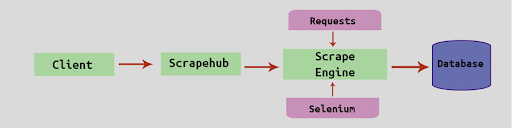
\includegraphics[width=15cm]{includes/webscraping.png}
	\centering
	\caption{ Traditional Web Scraper[43].}
	\label{fig:webscraping}
\end{figure}
The process of web scraping is a combination of two operations, first the web data extraction and next will be processing or cleaning the extracted raw data to provide insightful information. The data extraction part is easier when the source data is in the form of a database or an ontological structure but in most cases all web data extraction deals with unstructured or semi-structured data. Even now the researchers are coming up with new methods to improve the data scraping more efficiently and fast. In 2021 Jaebeom You et al[45] proposed a method called “DeepScrap” for collecting tweets. The DeepScrap method is used for scraping all the recent tweets in a fast speed by using Twitter’s standard API. The multiprocessing of deepScrap helps to get refined information rather than going with single processing. This scraping technique can help the OSS scanner to extract the name and version of a component.

{\bf Screen Scraping:} In short, screen scraping means reading text data from a computer terminal screen or a piece of programming that mediates legacy applications and modern user interfaces[47]. Both web scraping and screen scraping have many similarities, with the exception of a few key differences, such as where the data is gathered and how it is used. This scraper technique is mainly used for scanning old sources because of the quick speed of technological change, certain legacy systems, software, and applications become outdated and expensive to maintain. This would be a big and complicated process when the organization decides to migrate the old resource to the latest one without the help of a screen scraper. In 2017 there was a report where SnapLogic and the independent research firm Vanson Bourne stated that more than 500 U.S IT companies datas are completely trapped in their legacy system[46]. A \$140 million loss was incurred as a result of the data trap. It is not mandatory that every company should use screen scraping, this is more needed for companies like companies who hold their clients data for very long time record keeping purposes like companies who produce CRM services, crypto or stock exchanges, etc. Even without the source code of any legacy application, the screen scraper can still extract the data. 
\paragraph{}
Sergio Flores-Ruiz et al have explained black-box solution for the migration process of a mainframe by using screen scraping technique[49]. The author came up with a back-box solution to JavaFX and relational database mainframe systems because the majority of these legacy systems are consolidated on mainframes. The author also mentioned that the previous migrating solution was not that efficient due to a shortage of systematicity and lack of business rule verification. As we know, applying screen scraper technique to retrieve legacy information from an old source is an effective idea but there is some research which has tried to take the screen scraping next step. An operation of screen scraper is, once the information is retrieved from the legacy information system and it is moved to the new data storage system. After this operation the legacy information system will be deactivated by the organization. Alex van Oostenrijk[50] has tried to implement web service between a website and the legacy information system by using screen scraper technique. He believed that a continuous screen scraping system would be key to achieve it. Continuous screen scraping is nothing but keeping the old information system active and trying to connect the new system(website) with the help of web services. After the implementation, the author experienced that this is not a robust idea because it was taking four minutes to search 132 pages per request but it can be overcomed by using a caching technique.

\subsubsection{Challenges}

\subsubsection{Data Scraping Methods}
Mostly data scraping used purposes like marketing and price research, monitoring, analyzing and retrieving information for decision making and CRM tools. If a user or organization configures the data scraping technique effectively the tool will be quite powerful for retrieving meaningful information. The data scraping has been classified into two scraping techniques which will be utilised based on the requirements:

{\bf Manual Scraping:} As everyone knows, data scraping is mostly done automated but it can be also manually scraped from a resource. This is the traditional way of data scraping. This process is nothing but seeing through your vision and replicating it into desired format like a spreadsheet. The advantage of manual scraping is that it is very easy to implement, no need for any extra skills and human intervention. The same time manual scraping also has its drawbacks like when compared to automated scraping it is slow, high cost and with human intervention errors may occur. Under manual scraping there is only one technique available[51]:
\begin{description}
	\item [$\bullet$ Copy-Pasting:] In Manual scripting all the user wants to know is copy-pasting which takes a lot of effort. Most of the time the manual scripting will have data reputation issues because of human involvement. Manual scraping, on the other hand, is seldom seen in reality because automated scraping is considerably faster and less expensive.
\end{description}

{\bf Automated  Scraping:} The evolution of manual scraping is automated scraping, the current IT era is moving through automation to reduce human effort  and to make it cost effective with high accuracy. Because of their simplicity of use and time and cost advantages, automated web scraping technologies have grown in popularity. Automated scraping has more advantages than manual scripting like very fast data scraping and extraction, time and cost efficiency, easy to use and supports API services. Eventually it also has its negative side which is not that bad like requiring light training, in some cases scraping is illegal and lacks human checks. Automated scraping has many methods to scrape data based on the requirement:
\begin{description}
	\item [$\bullet$ HTML Parsing:] This is the easiest and fastest way of extracting data from a file. This technique is mainly used for extracting data from the html files. The parsing is done with the help of a programming language like JavaScript to extract data from the html file. 
	
	\item [$\bullet$ DOM Parsing:] The document model object is an interface which is used to parse XML or html file source code into string. The main purpose of the DOM parser is to get the in-depth structure of the html or xml file. The representation of a document is shown in tree view. With the help of a DOM parser the scrapper can extract the information from the node data. The positive side of the dom parser is more effective than normal parsing methods like the data persisting in the memory, forward and backward traversing is possible and direct changes are possible.
	\item [$\bullet$ XPath:] XPath stands for XML path and its an exclusive querying language for XML files. The xpath is used to navigate across the xml file because the xml documents are based on tree structure. There are few reasons why xpath is preferable when parsing xml file like, the queries are compact, easy to use, simple syntax, do not return repeated values and work with both html and xml attributes. Due to its interoperability the xpath can be used any programming language like C, C++, C-Sharp, Java, Javascript, etc. Xpath also has the potential to retrieve the relevant information from any complicated xml file by allowing different types of expressions. The important expressions are, Root, Element, Attribute, Text and Comment.
	\item [$\bullet$ Text Pattern Matching:] Pattern matching is a powerful tool for extracting information from natural language. It can be used to perform tasks from simple text segmentation, to complex parsing and machine translation. In technical terms it is a process of verifying the given sequence of characters to find similarities with a pattern. The patterns to verify the given string are designed or created by the help of regular expression. The regular expression is supported by most programming languages. Unlike other methods the pattern matching can be implied on all data types. Pattern matching can be performed simultaneously with the help of parallel pattern matching. 
\end{description}
\subsection{String Distance Metrics}
Both supervised and unsupervised learning can benefit from distance measures. Distance measurements can be used for text mining, medical analysis, document categorization, and similarity analysis, among other things. The main purpose of string metrics is to correct a spelling mistake by calculating the distance between two data points or string, the calculation will give the string similarity between the given inputs. In simpler terms, it is a process of calculating distance between one text to another text to find similarity. Till now the string metrics are frequently used as information integration in areas like fraudulent detection, fingerprint analysis, plagiarism detection, ontology merging, DNA analysis, RNA analysis, image analysis, etc. The distance between strings may be calculated using a variety of algorithms. Each algorithm calculates the distance between strings but apart from this it also has some unique features. The following algorithms are:
\subsubsection{Hamming Distance}
Hamming distance is a simpler algorithm to calculate distance between two strings which was found by Richard Hamming who introduced this technique for Hamming codes. The algorithm performs  calculation to find the similarity in the given strings by comparing the changes in the position of the two strings[52].

\begin{figure}[h!]
	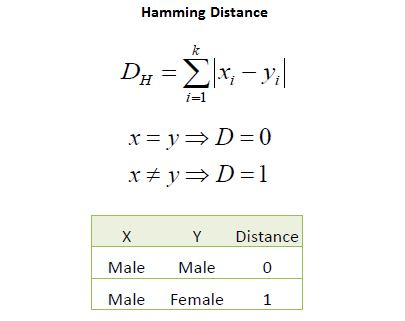
\includegraphics[width=10cm]{includes/hamming.png}
	\centering
	\caption{ Hamming Distance Formula[53].}
	\label{fig:hamming}
\end{figure}
Figure 3.1 explains how the distance is calculated between the two strings sto find the similarity. The benefits of using hamming distance are it is simpler and effective to detect spelling mistakes or errors. They are also quite good and effective in data streams. The only disadvantage of using hamming distance is that the bandwidth usage is more.
\subsubsection{Levenshtein distance}
e Levenshtein distance algorithm is also used to find the distance between two strings along with a few operations to it. The algorithm was discovered by Vladimir Levenshtein from Russia. The Levenshtein distance is also known as the Edit-distance based algorithm because it computes the number of edits to find the distance. The edit contains three operations which are Insertionation, Deletion and Substitution. To find less similarity between two strings, it requires more operation[54]. For example the distance between GILY and GEELY is 2 and two operations have been done which are substitution and deletion.

\begin{figure}[h!]
	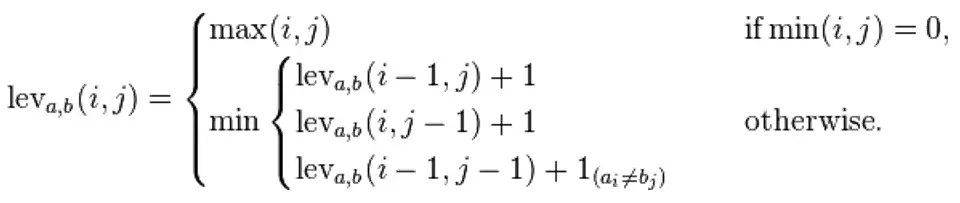
\includegraphics[width=10cm]{includes/levdist.png}
	\centering
	\caption{ Levenshtein distance Formula.}
	\label{fig:levdist}
\end{figure}
The algorithm can be used for word suggestion and autocorrection by measuring how different two strings are by counting the number of character edits. Implementing the Levenshtein distance algorithm as a recursive implementation will cause massive complexity but this can be solved by using a proper memoization technique.

\subsubsection{Damerau-Levenshtein distance}
The Damerau-Levenshtein distance algorithm is an updated version of the Levenshtein distance algorithm. The one difference which separates  Damerau-Levenshtein from Levenshtein is that it includes another operation: transposition. It takes only a minimum number of operations to find the similarity of the strings by changing one word to another. The name Damerau-Levenshtein was derived from the scientists Frederick J. Damerau and Vladimir I. Levenshtein. The main benefit of using the Damerau-Levenshtein algorithm is that it is comparatively faster than its predecessor algorithm and it also saves time by avoiding Regex expression to calculate the similarity[55]. 

\begin{figure}[h!]
	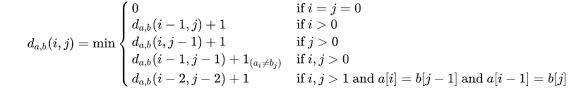
\includegraphics[width=10cm]{includes/dlevidist.png}
	\centering
	\caption{ Damerau-Levenshtein Distance formula[56].}
	\label{fig:dlevidist}
\end{figure}
In natural language processing, the Damerau–Levenshtein distance is a crucial factor. They are mainly considered in the area of DNA analysis and Fraudulent detection.
\subsubsection{Jaro Distance}
Jaro distance is a metric for comparing the similarity of two strings and it is defined using this formula.

\begin{figure}[h!]
	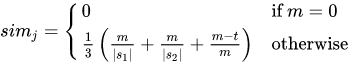
\includegraphics[width=10cm]{includes/jaro.png}
	\centering
	\caption{ Jaro similarity formula[57].}
	\label{fig:jaro}
\end{figure}
Here s1 and s2 are the two strings. m is considered as the number of matching characters and t is considered as half the number of matching characters. Unlike the other string distance algorithm, the Jaro distance ranges from 0 to 1 where 0 means no similarity and 1 has similarity[58]. The result of the algorithm will be given as a float value.This can be used to check whether the two strings are the same or not. 
The improved version of the Jaro similarity algorithm is the Jaro-Winkler distance algorithm. The Jaro-Winkler algorithm is also similar to Jaro similarity but the Winkler is built using prefix scale p for finding precise distance.

\begin{figure}[h!]
	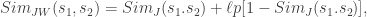
\includegraphics[width=10cm]{includes/jarowinkler.png}
	\centering
	\caption{ Jaro-Winkler similarity formula[59].}
	\label{fig:jarowinkler}
\end{figure}